\chapter{TINJAUAN PUSTAKA}
\label{chap:tinjauanpustaka}

% Ubah bagian-bagian berikut dengan isi dari tinjauan pustaka

Demi mendukung penelitian ini, dibutuhkan beberapa teori penunjang sebagai bahan acuan dan refrensi. Dengan demikian penelitian ini menjadi lebih terarah.

\section{Dasar Teori}
\label{sec:dasarteori}

\subsection{\textit{Artificial Intelligence}}
\label{artificialintelligence}

\textit{Artificial Intelligence} mengacu pada simulasi kecerdasan manusia dalam mesin yang diprogram untuk berpikir seperti manusia dan meniru tindakan mereka.\citep{artificialintellingece} Istilah ini juga dapat diterapkan pada mesin apa pun yang menunjukkan ciri-ciri yang terkait dengan pikiran manusia seperti pembelajaran dan pemecahan masalah.

Karakteristik ideal dari \textit{artificial intellingence} adalah kemampuannya untuk merasionalisasi dan mengambil tindakan yang memiliki peluang terbaik untuk mencapai tujuan tertentu. Bagian dari \textit{artificial intellingece} adalah \textit{machine learning}, yang mengacu pada konsep bahwa program komputer dapat secara otomatis belajar dari dan beradaptasi dengan data baru tanpa dibantu oleh manusia. Teknik\textit{deep learning} memungkinkan pembelajaran otomatis ini melalui penyerapan sejumlah besar data tidak terstruktur seperti teks, gambar, atau video.

\subsection{\textit{Machine Learning}}
\label{machinelearning}

\textit{Machine Learning} adalah studi tentang algoritma komputer yang memberikan sistem kemampuan untuk belajar secara otomatis dan dapat meningkatkan kemampuan dari pengalaman yang sudah didapatkan \citep{machinelearning1}. Hal ini umumnya dilihat sebagai sub-bidang kecerdasan buatan. Algoritma pembelajaran mesin memungkinkan sistem membuat keputusan secara mandiri tanpa dukungan eksternal. Keputusan semacam itu dibuat dengan menemukan pola dasar yang berharga dalam data yang kompleks. Berdasarkan pendekatan pembelajaran, jenis data \textit{input} dan \textit{output}, dan jenis masalah yang dipecahkan, ada beberapa kategori utama dari algoritma \textit{machine learning} \textit{supervised, unsupervised} dan \textit{reinforcement learning}. Ada beberapa pendekatan hibrida dan metode umum lainnya yang menawarkan ekstrapolasi alami dari bentuk masalah pembelajaran mesin. Berikut merupakan penjelasan dari beberapa kategori utama dari algoritma \textit{machine learning}:

\begin{enumerate}
	\item \textit{Supervised Learning} diterapkan ketika data dalam bentuk variabel input dan nilai target output. Algoritma akan mempelajari fungsi pemetaan dari \textit{input} ke \textit{output}. Ketersediaan sampel data berlabel dengan skala besar mempunyai nilai yang tinggi dikarenakan masih terdapat kelangkaan \textit{dataset}. Pendekatan ini secara luas dapat dibagi menjadi dua kategori utama yaitu \textit{classification} dan \textit{regression}. Gambar \ref{fig:supervised} menampilkan visualisasi dari \textit{classification} dan \textit{regression} pada \textit{Supervised Learning}
	
	\begin{figure}[ht]
		\centering
		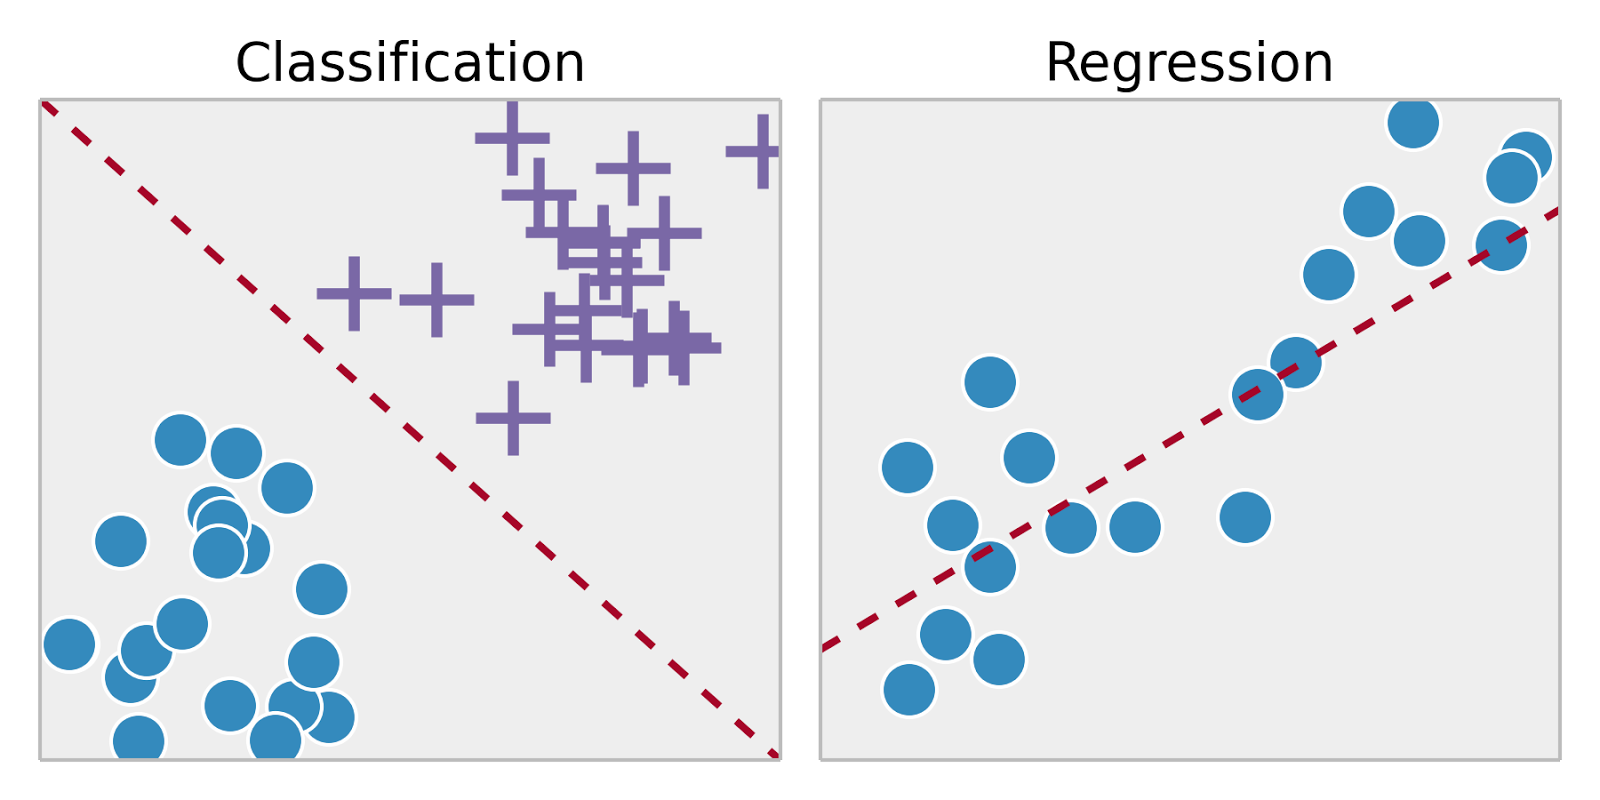
\includegraphics[scale=0.1]{gambar/supervised.png}
		\caption{Gambaran \textit{Supervised Learning}\citep{supervised}}
		\label{fig:supervised}
	\end{figure}  
	
	\item \textit{Unsupervised Learning} diterapkan ketika data hanya tersedia dalam bentuk \textit{input} dan tidak ada variabel \textit{output} yang sesuai. Algoritma semacam itu memodelkan pola yang mendasari data untuk mempelajari lebih lanjut tentang karakteristiknya. Salah satu jenis utama dari algoritma \textit{unsupervised} adalah pengelompokan. Dalam teknik ini, kelompok yang melekat dalam data ditemukan dan kemudian digunakan untuk memprediksi \textit{output} untuk \textit{input} yang tidak terlihat. Contoh dari teknik ini adalah untuk memprediksi perilaku pembelian pada pelanggan. Gambar \ref{fig:unsupervised} merupakan visualisasi dari algoritma \textit{unsupervised learning}.
	
	\begin{figure}[ht]
		\centering
		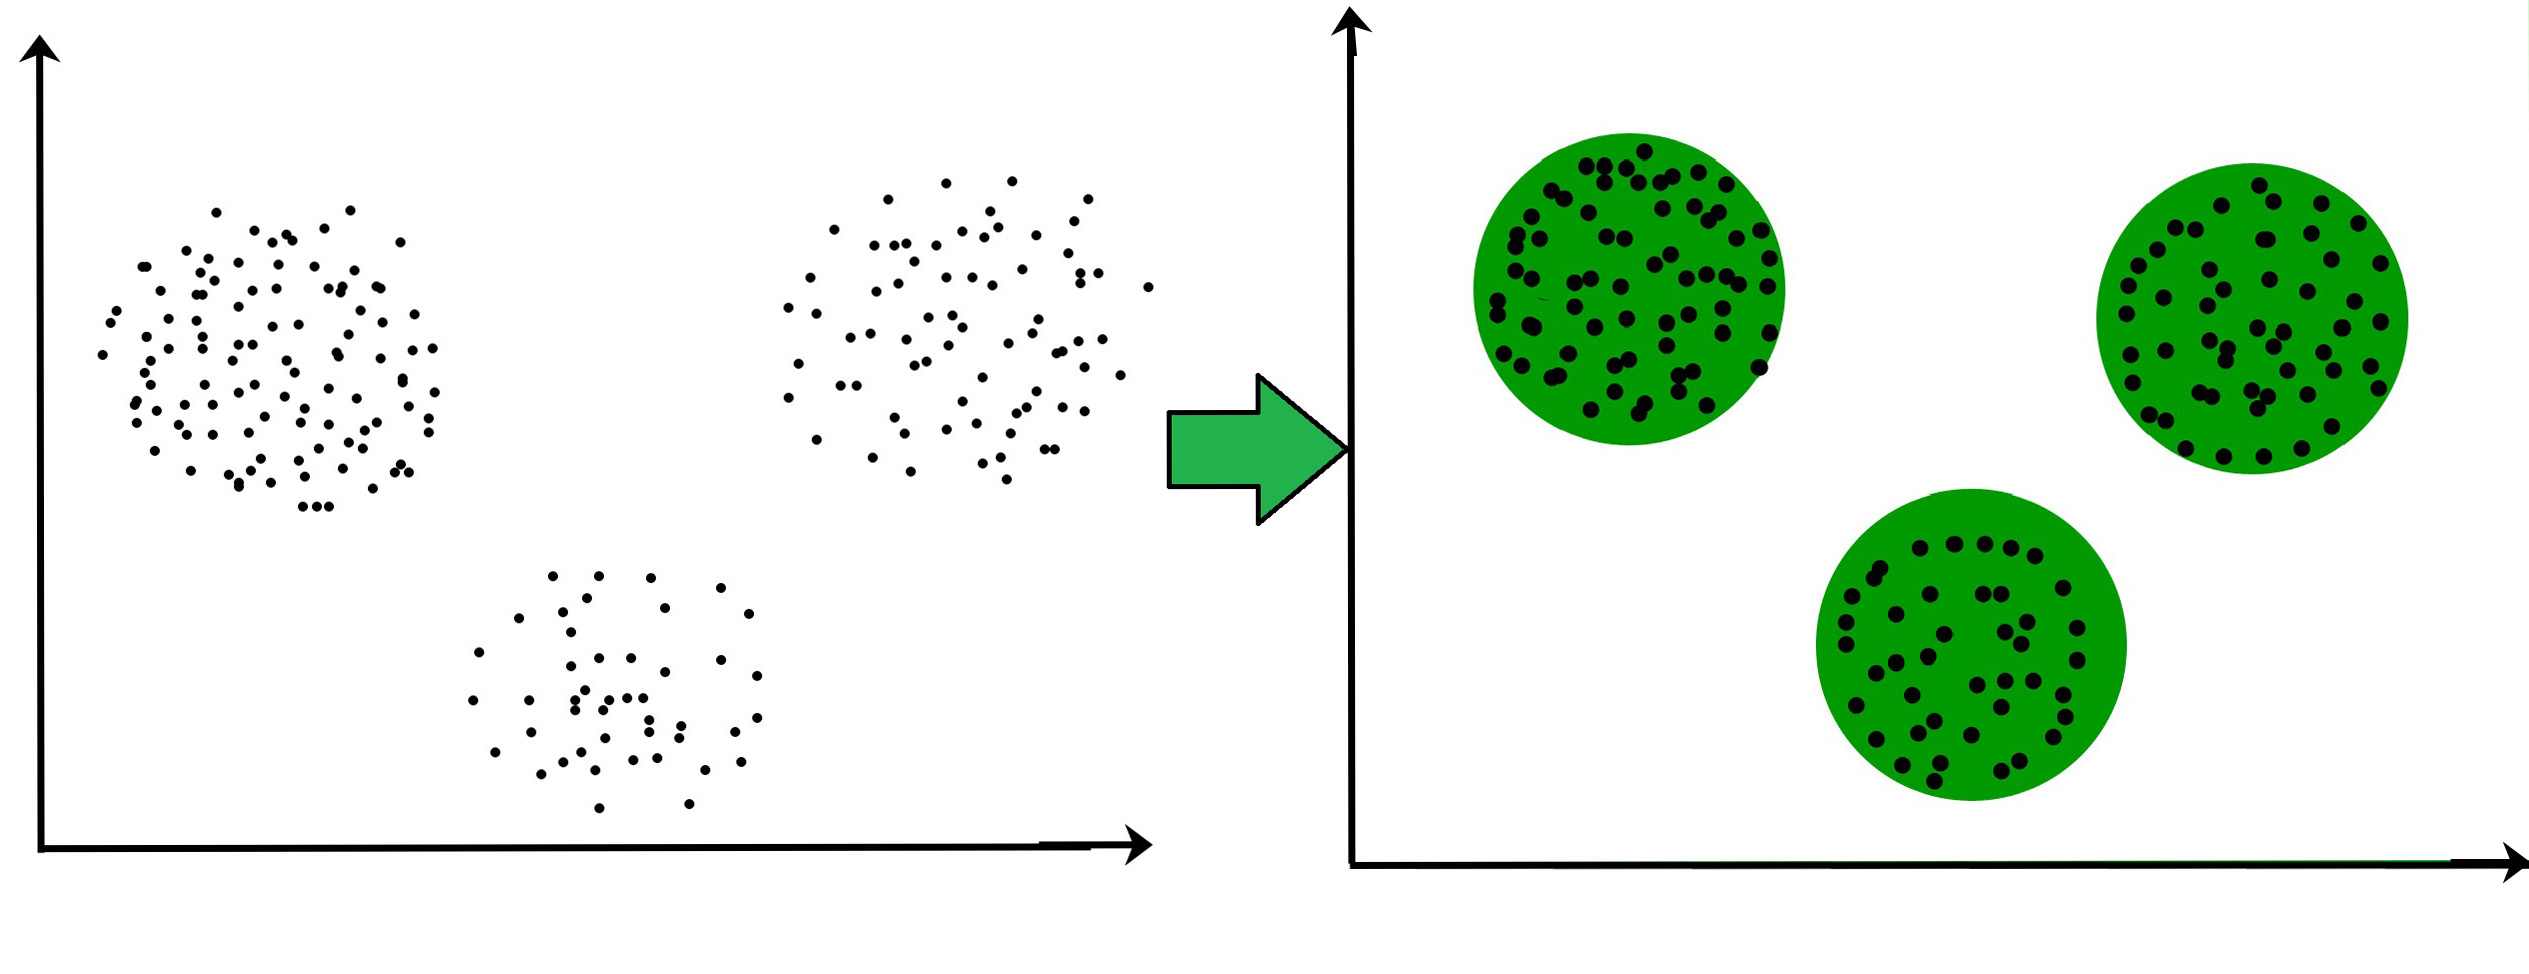
\includegraphics[scale=0.2]{gambar/unsupervised.jpg}
		\caption{Gambaran \textit{Unsupervised Learning}\citep{unsupervised}}
		\label{fig:unsupervised}
	\end{figure}
	
	
	\item \textit{Reinforcement learning} diterapkan ketika tugas yang ada
	adalah membuat urutan keputusan menuju \textit{reward} akhir. Selama proses \textit{learning}, \textit{artificial agent} mendapat \textit{reward} atau \textit{penalties} atas tindakan yang dilakukannya. Tujuannya adalah untuk memaksimalkan total \textit{reward} yang didapatkan. Gambar \ref{fig:reinforcement} merupakan visualisasi dari algoritma \textit{reinforcement learning}.
	
	\begin{figure}[ht]
		\centering
		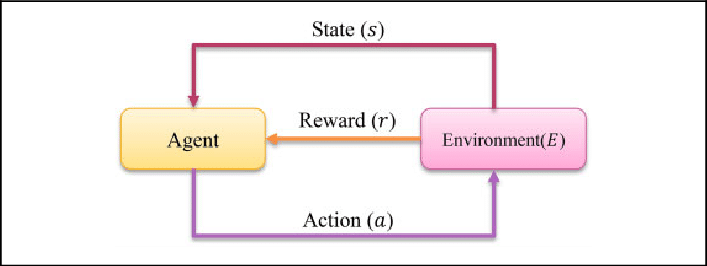
\includegraphics[scale=0.3]{gambar/reinforcement.png}
		\caption{Gambaran \textit{Reinforcement Learning}\citep{reinforcement}}
		\label{fig:reinforcement}
	\end{figure}
\end{enumerate}

\subsection{\textit{Deep Learning}}
\label{deeplearning}

\textit{Deep Learning} adalah kelas \textit{machine learning} yang berkinerja jauh lebih baik pada data tidak terstruktur\citep{dl}. Teknik \textit{deep learning} mengungguli teknik \textit{machine learning} saat ini. Ini memungkinkan model komputasi untuk mempelajari fitur secara progresif dari data di berbagai level. Popularitas \textit{deep learning} diperkuat karena jumlah data yang tersedia meningkat serta kemajuan perangkat keras yang menyediakan komputer yang kuat.

Arsitektur \textit{deep learning} berkinerja lebih baik daripada jaringan saraf tiruan  sederhana, meskipun waktu \textit{learning} dari struktur \textit{deep learning} lebih tinggi dari jaringan saraf tiruan. Namun, waktu \textit{learning} dapat dikurangi dengan menggunakan metode seperti \textit{transfer learning} atau komputasi menggunakan GPU. Salah satu faktor yang menentukan keberhasilan jaringan saraf terletak pada desain arsitektur jaringan yang cermat.

\subsection{\textit{Convolutional Neural Network}}
\label{cnn}

\textit{Convolutional Neural Networl} (CNN) adalah jenis khusus dari \textit{multilayer neural network} atau arsitektur \textit{deep learning} yang terinspirasi oleh sistem visual makhluk hidup \citep{cnn}. CNN sangat cocok untuk berbagai bidang visi komputer dan \textit{natural language processing}. \textit{Convolutional Neural Network} (CNN), juga disebut \textit{ConvNet}, adalah jenis \textit{Artificial Neural Network} (ANN), yang memiliki arsitektur \textit{feed-forward} yang dalam dan memiliki kemampuan generalisasi yang luar biasa dibandingkan dengan jaringan lain dengan lapisan FC (\textit{Fully Connected}), ia dapat mempelajari fitur objek yang sangat abstrak terutama data spasial dan dapat mengidentifikasinya dengan lebih efisien. Model CNN yang dalam terdiri dari satu set lapisan pemrosesan yang dapat mempelajari berbagai fitur data \textit{input} (misalnya gambar) dengan beberapa tingkat abstraksi seperti yang ditampilkan pada Gambar \ref{fig:concept-cnn}. Lapisan inisiator mempelajari dan mengekstrak fitur tingkat tinggi (dengan abstraksi yang lebih rendah), dan lapisan yang lebih dalam mempelajari dan mengekstrak fitur tingkat rendah (dengan abstraksi yang lebih tinggi).

\begin{figure}[ht]
	\centering
	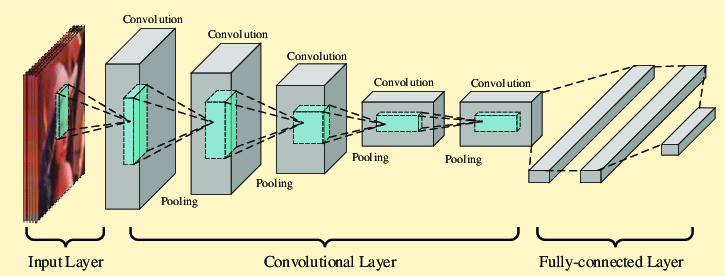
\includegraphics[scale=0.3]{gambar/concept-cnn.png}
	\caption{Gambaran Konsep Arsitektur CNN \citep{concept-cnn}}
	\label{fig:concept-cnn}
\end{figure}